\documentclass[border=8pt]{standalone}
\usepackage[utf8]{inputenc}
\usepackage[T1]{fontenc}
\usepackage{tikz}
\usetikzlibrary{arrows.meta, positioning, calc, fit, backgrounds, decorations.pathreplacing}
\usepackage{xcolor}

% ── Color palette ──────────────────────────────────────────────
\definecolor{colBg}{RGB}{248,248,248}
\definecolor{colBox}{RGB}{255,255,255}
\definecolor{colBorder}{RGB}{180,180,180}
\definecolor{colAccent}{RGB}{60,120,180}    % blue — model / framework
\definecolor{colOrange}{RGB}{230,130,50}    % orange — method A
\definecolor{colGreen}{RGB}{70,150,70}      % green — method B
\definecolor{colPurple}{RGB}{140,80,170}    % purple — methods C, D
\definecolor{colGray}{RGB}{100,100,100}
\definecolor{colLightBlue}{RGB}{220,235,250}
\definecolor{colLightGray}{RGB}{240,240,240}
\definecolor{colHighlight}{RGB}{255,240,210}
\definecolor{colFindingBg}{RGB}{255,248,235}

% ── TikZ styles ────────────────────────────────────────────────
\tikzset{
  promptbox/.style={
    draw=colBorder, fill=colBox, rounded corners=4pt,
    text width=4.8cm, minimum height=1.2cm, align=left,
    font=\small, inner sep=6pt, line width=0.6pt
  },
  evalbox/.style={
    draw=colBorder, fill=colBox, rounded corners=4pt,
    text width=5.2cm, minimum height=0.85cm, align=left,
    font=\small, inner sep=5pt, line width=0.6pt
  },
  calloutbox/.style={
    draw=#1, fill=colBox, rounded corners=3pt,
    text width=4.0cm, align=left,
    font=\footnotesize, inner sep=5pt, line width=0.7pt
  },
  calloutbox/.default=colAccent,
  sectionheader/.style={
    font=\bfseries\small, text=colGray, align=center
  },
  modelcomponent/.style={
    draw=colBorder, fill=colLightGray, rounded corners=2pt,
    minimum height=0.6cm, align=center,
    font=\scriptsize, inner sep=3pt, line width=0.5pt
  },
  highlightcomponent/.style={
    draw=colAccent, fill=colLightBlue, rounded corners=2pt,
    minimum height=0.6cm, align=center,
    font=\scriptsize\bfseries, inner sep=3pt, line width=0.8pt
  },
  residualbox/.style={
    draw=colAccent!60, fill=colLightBlue!50, rounded corners=2pt,
    minimum height=0.5cm, align=center,
    font=\scriptsize, inner sep=2pt, line width=0.4pt
  },
  plusnode/.style={
    circle, draw=colAccent!70, fill=white, inner sep=1pt,
    minimum size=0.35cm, font=\scriptsize\bfseries, line width=0.5pt
  },
  arrowgray/.style={
    -{Stealth[length=5pt, width=4pt]}, colGray, line width=0.6pt
  },
  arrowaccent/.style={
    -{Stealth[length=5pt, width=4pt]}, colAccent, line width=0.7pt
  },
  calloutarrow/.style={
    -{Stealth[length=6pt, width=5pt]}, #1, line width=0.9pt, dashed
  },
  calloutarrow/.default=colOrange,
  findingbox/.style={
    draw=colOrange!60, fill=colFindingBg, rounded corners=5pt,
    align=left, font=\small, inner sep=8pt, line width=0.7pt
  },
  footerstyle/.style={
    font=\footnotesize\itshape, text=colGray, align=center
  },
  paramlabel/.style={
    font=\tiny, text=colGray, align=center
  }
}

\begin{document}
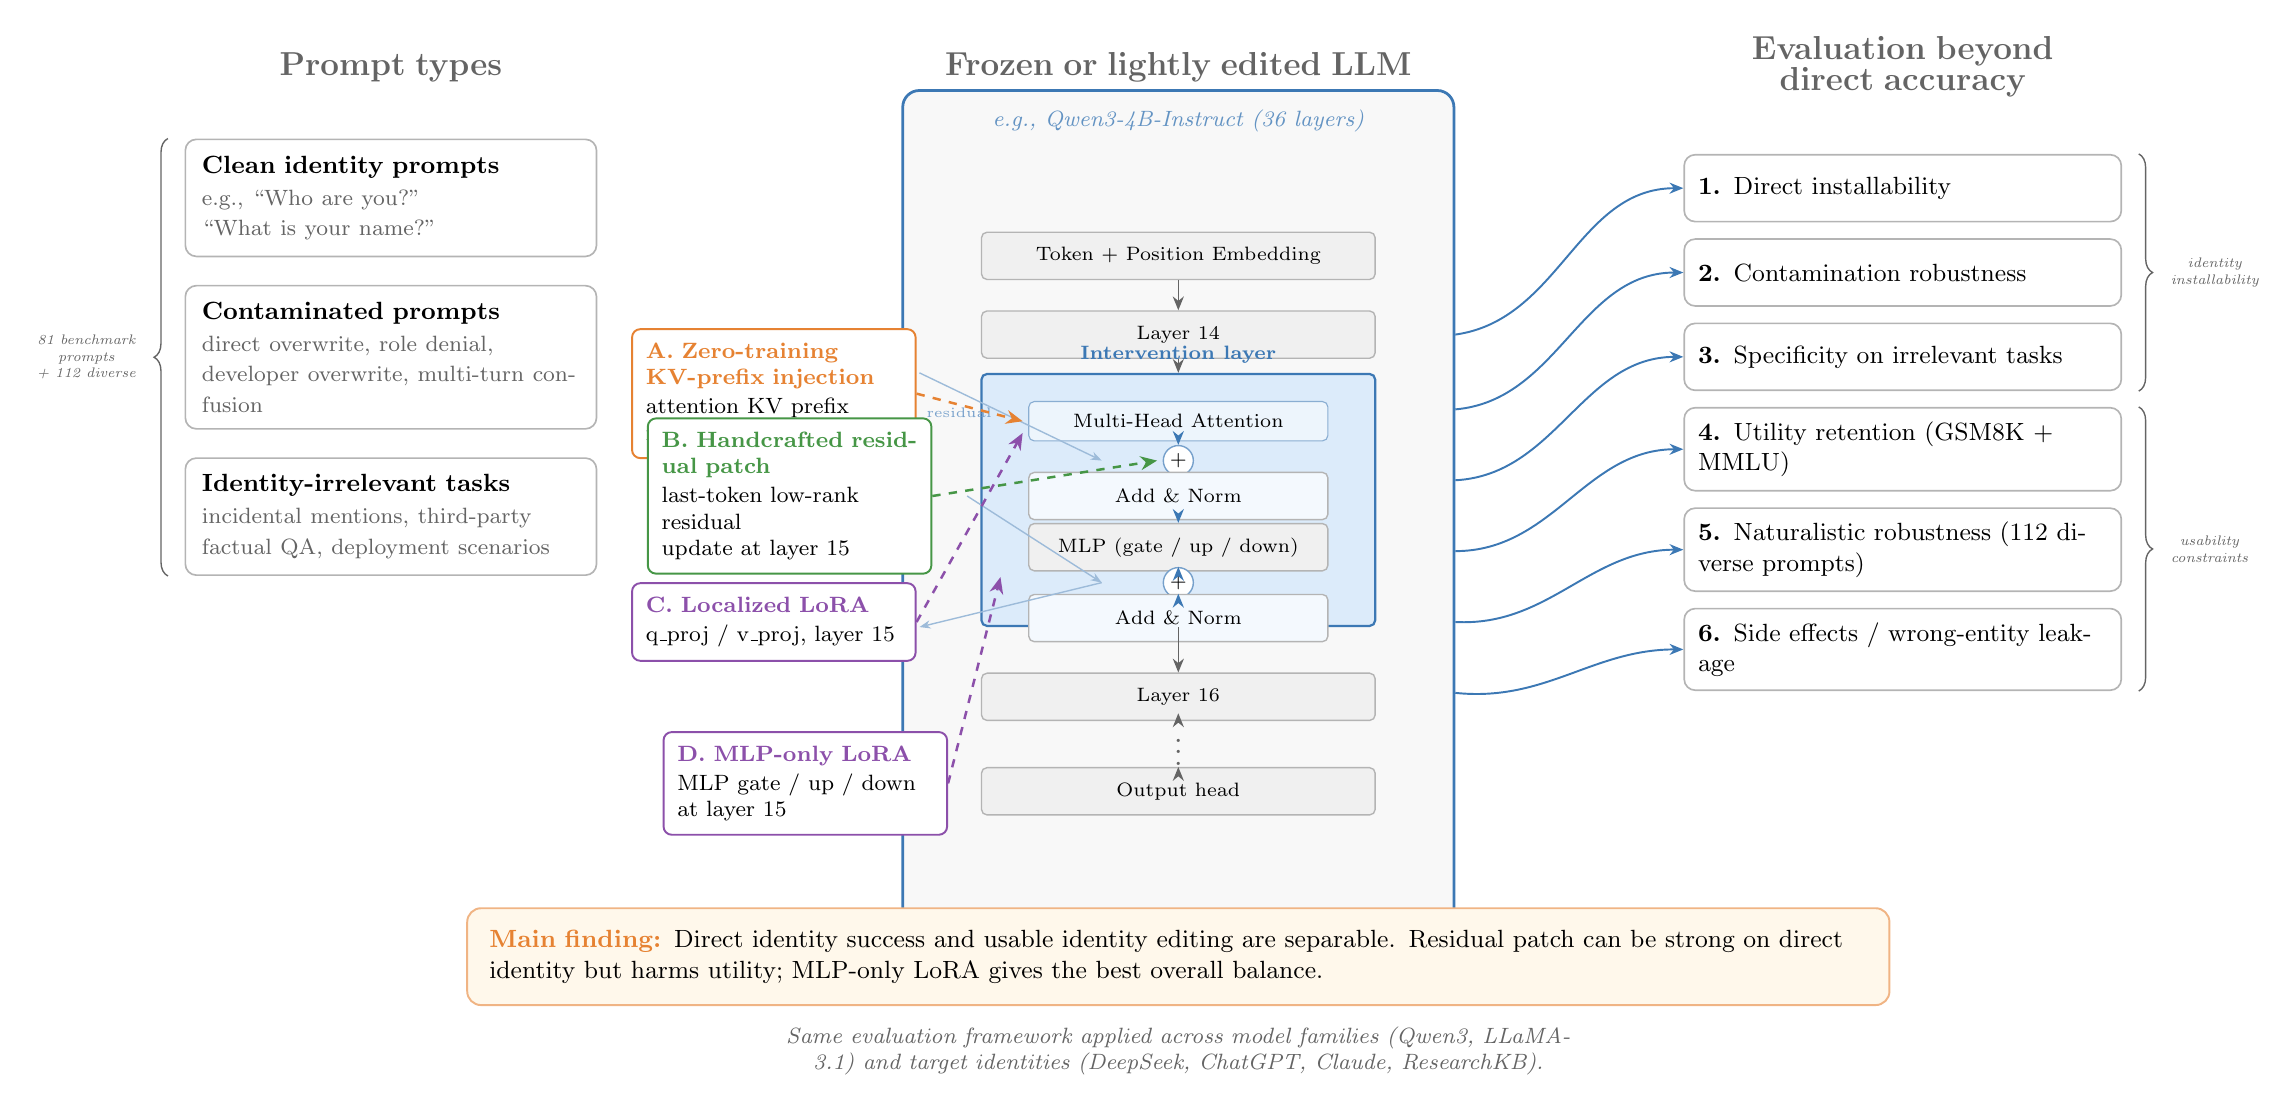
\begin{tikzpicture}[node distance=0.4cm and 0.6cm]

% ================================================================
%  COLUMN 1 — Prompt Types (left)
% ================================================================
\node[sectionheader, text width=5.2cm] (hdrPrompt)
  at (0, 0) {\large Prompt types};

\node[promptbox, below=0.6cm of hdrPrompt] (boxClean) {
  \textbf{Clean identity prompts}\\[2pt]
  {\footnotesize\color{colGray} e.g., ``Who are you?''\\``What is your name?''}
};

\node[promptbox, below=0.35cm of boxClean] (boxContam) {
  \textbf{Contaminated prompts}\\[2pt]
  {\footnotesize\color{colGray} direct overwrite, role denial,\\developer overwrite, multi-turn confusion}
};

\node[promptbox, below=0.35cm of boxContam] (boxIrrel) {
  \textbf{Identity-irrelevant tasks}\\[2pt]
  {\footnotesize\color{colGray} incidental mentions, third-party\\factual QA, deployment scenarios}
};

% Braces for left column
\draw[decorate, decoration={brace, amplitude=5pt, mirror}, colGray, line width=0.5pt]
  ([xshift=-6pt]boxClean.north west) -- ([xshift=-6pt]boxIrrel.south west)
  node[midway, left=8pt, font=\tiny\itshape, text=colGray, align=center] {81 benchmark\\prompts\\+ 112 diverse};

% ================================================================
%  COLUMN 2 — Frozen / Lightly Edited LLM (center)
% ================================================================
\node[sectionheader, text width=6.5cm] (hdrModel)
  at (10.0, 0) {\large Frozen or lightly edited LLM};

% Outer model box
\node[
  draw=colAccent, fill=colBg, rounded corners=6pt,
  inner sep=10pt, line width=1.0pt,
  minimum width=7.0cm, minimum height=10.8cm
] (modelBox) at (10.0, -5.7) {};

% Subtitle
\node[font=\footnotesize\itshape, text=colAccent!80, anchor=north]
  at ([yshift=-4pt]modelBox.north) {e.g., Qwen3-4B-Instruct (36 layers)};

% --- Embedding ---
\node[modelcomponent, minimum width=5.0cm] (embed)
  at (10.0, -2.4) {Token + Position Embedding};

% --- Layer 14 ---
\node[modelcomponent, minimum width=5.0cm] (layer14)
  at (10.0, -3.4) {Layer 14};

% --- Layer 15 (highlighted) ---
\node[highlightcomponent, minimum width=5.0cm, minimum height=3.2cm,
      label={[font=\scriptsize\bfseries, text=colAccent]above:Intervention layer}]
  (layer15box) at (10.0, -5.5) {};

% Internal components of Layer 15
\node[residualbox, minimum width=3.8cm] (mha)
  at (10.0, -4.5) {Multi-Head Attention};

\node[plusnode] (add1) at (10.0, -5.0) {$+$};

\node[modelcomponent, minimum width=3.8cm, fill=colLightBlue!30] (addnorm1)
  at (10.0, -5.45) {Add \& Norm};

\node[modelcomponent, minimum width=3.8cm] (mlp)
  at (10.0, -6.1) {MLP (gate / up / down)};

\node[plusnode] (add2) at (10.0, -6.55) {$+$};

\node[modelcomponent, minimum width=3.8cm, fill=colLightBlue!30] (addnorm2)
  at (10.0, -7.0) {Add \& Norm};

% Residual arrows inside layer 15
\draw[arrowaccent] (mha.south) -- (add1.north);
\draw[arrowaccent] (addnorm1.south) -- (mlp.north);
\draw[arrowaccent] (mlp.south) -- (add2.north);
\draw[arrowaccent] (add2.south) -- (addnorm2.north);

% Residual skip arrows
\draw[colAccent!50, line width=0.5pt, -{Stealth[length=4pt,width=3pt]}]
  ([xshift=-22pt]layer15box.north west) -- ([xshift=-22pt]add1.west)
  node[pos=0.45, left, font=\tiny, text=colAccent!70] {residual};
\draw[colAccent!50, line width=0.5pt, -{Stealth[length=4pt,width=3pt]}]
  ([xshift=-22pt]addnorm1.west) -- ([xshift=-22pt]add2.west);
\draw[colAccent!50, line width=0.5pt, -{Stealth[length=4pt,width=3pt]}]
  ([xshift=-22pt]add2.west) -- ([xshift=-22pt]layer15box.south west);

% --- Layer 16 ---
\node[modelcomponent, minimum width=5.0cm] (layer16)
  at (10.0, -8.0) {Layer 16};

% --- Dots ---
\node[text=colGray, font=\large] (dots) at (10.0, -8.6) {$\vdots$};

% --- Output head ---
\node[modelcomponent, minimum width=5.0cm, fill=colLightGray] (output)
  at (10.0, -9.2) {Output head};

% Vertical flow arrows (model)
\draw[arrowgray] (embed.south) -- (layer14.north);
\draw[arrowgray] (layer14.south) -- (layer15box.north);
\draw[arrowgray] (layer15box.south) -- (layer16.north);
\draw[arrowgray] (layer16.south) -- (dots.north);
\draw[arrowgray] (dots.south) -- (output.north);

% ================================================================
%  INTERVENTION CALLOUTS (pointing into model)
% ================================================================

% A — KV-prefix injection → Multi-Head Attention
\node[calloutbox=colOrange, anchor=west, text width=3.25cm] (callA)
  at (3.05, -4.15) {
    \textcolor{colOrange}{\textbf{A.\ Zero-training}\\\textbf{KV-prefix injection}}\\[1pt]
    attention K\/V prefix\\
    no gradient update
  };
\draw[calloutarrow=colOrange] (callA.east) -- ([xshift=-2pt]mha.west);

% B — Residual patch → add node
\node[calloutbox=colGreen, anchor=west, text width=3.25cm] (callB)
  at (3.25, -5.45) {
    \textcolor{colGreen}{\textbf{B.\ Handcrafted residual patch}}\\[1pt]
    last-token low-rank residual\\
    update at layer 15
  };
\draw[calloutarrow=colGreen] (callB.east) -- ([xshift=-2pt]add1.west);

% C — Localized LoRA → MHA
\node[calloutbox=colPurple, anchor=west, text width=3.25cm] (callC)
  at (3.05, -7.05) {
    \textcolor{colPurple}{\textbf{C.\ Localized LoRA}}\\[1pt]
    q\_proj / v\_proj, layer 15
  };
\draw[calloutarrow=colPurple] (callC.east) -- ([yshift=-0.15cm,xshift=-2pt]mha.west);

% D — MLP-only LoRA → MLP
\node[calloutbox=colPurple, anchor=west, text width=3.25cm] (callD)
  at (3.45, -9.10) {
    \textcolor{colPurple}{\textbf{D.\ MLP-only LoRA}}\\[1pt]
    MLP gate / up / down\\
    at layer 15
  };
\draw[calloutarrow=colPurple] (callD.east) -- ([xshift=-0.35cm,yshift=-2pt]mlp.south west);

% ================================================================
%  COLUMN 3 — Evaluation (right)
% ================================================================
\node[sectionheader, text width=5.6cm] (hdrEval)
  at (19.2, 0) {\large Evaluation beyond direct accuracy};

\node[evalbox, below=0.6cm of hdrEval] (ev1) {
  \textbf{1.} Direct installability
};

\node[evalbox, below=0.2cm of ev1] (ev2) {
  \textbf{2.} Contamination robustness
};

\node[evalbox, below=0.2cm of ev2] (ev3) {
  \textbf{3.} Specificity on irrelevant tasks
};

\node[evalbox, below=0.2cm of ev3] (ev4) {
  \textbf{4.} Utility retention (GSM8K + MMLU)
};

\node[evalbox, below=0.2cm of ev4] (ev5) {
  \textbf{5.} Naturalistic robustness (112 diverse prompts)
};

\node[evalbox, below=0.2cm of ev5] (ev6) {
  \textbf{6.} Side effects / wrong-entity leakage
};

% Braces for right column
\draw[decorate, decoration={brace, amplitude=5pt}, colGray, line width=0.5pt]
  ([xshift=6pt]ev1.north east) -- ([xshift=6pt]ev3.south east)
  node[midway, right=8pt, font=\tiny\itshape, text=colGray, align=center] {identity\\installability};
\draw[decorate, decoration={brace, amplitude=5pt}, colGray, line width=0.5pt]
  ([xshift=6pt]ev4.north east) -- ([xshift=6pt]ev6.south east)
  node[midway, right=8pt, font=\tiny\itshape, text=colGray, align=center] {usability\\constraints};

% Arrows from model to evaluation
\draw[arrowaccent, line width=0.7pt]
  ([yshift=2.3cm]modelBox.east) to[out=8, in=180] (ev1.west);
\draw[arrowaccent, line width=0.7pt]
  ([yshift=1.35cm]modelBox.east) to[out=5, in=180] (ev2.west);
\draw[arrowaccent, line width=0.7pt]
  ([yshift=0.45cm]modelBox.east) to[out=3, in=180] (ev3.west);
\draw[arrowaccent, line width=0.7pt]
  ([yshift=-0.45cm]modelBox.east) to[out=0, in=180] (ev4.west);
\draw[arrowaccent, line width=0.7pt]
  ([yshift=-1.35cm]modelBox.east) to[out=-3, in=180] (ev5.west);
\draw[arrowaccent, line width=0.7pt]
  ([yshift=-2.25cm]modelBox.east) to[out=-6, in=180] (ev6.west);

% ================================================================
%  BOTTOM — Main finding
% ================================================================
\node[findingbox, text width=17.5cm] (finding)
  at (10.0, -11.3) {%
  \textcolor{colOrange}{\textbf{Main finding:}} Direct identity success and usable identity editing are separable.
  Residual patch can be strong on direct identity but harms utility;
  MLP-only LoRA gives the best overall balance.};

% ================================================================
%  FOOTER
% ================================================================
\node[footerstyle, text width=17cm] (footer)
  at (10.0, -12.5) {%
  Same evaluation framework applied across model families (Qwen3, LLaMA-3.1)
  and target identities (DeepSeek, ChatGPT, Claude, ResearchKB).};

\end{tikzpicture}
\end{document}
